\chapter{Compositional Embeddings of Domain-Specific Languages} \label{ch:embedding}

This chapter presents the second case study: compositional embeddings of
domain-specific languages (DSLs). We concentrate on how to embed DSLs in a
modular way and compose them to build larger DSLs. We start with an introduction
to the problem that we aim to solve in \autoref{sec:problem}. Then we
demonstrate existing embedding techniques in \autoref{sec:embed} and show in
\autoref{sec:lang} that \emph{compositional embeddings} combine the advantages
of shallow and deep embeddings and surpasses other techniques like tagless-final
embeddings by supporting modular dependencies. We validate our approach by
showcasing a compositionally embedded DSL for document authoring in
\autoref{sec:dsl} and further evaluating it in \autoref{sec:evaluation}.

\section{Introduction} \label{sec:problem}

A common approach to defining DSLs is via a direct embedding into a host
language. This approach is used in several programming languages, such as
Haskell, Scala, and Racket. In those languages, various DSLs -- including pretty
printers~\citep{hughes1995design,wadler2003prettier}, parser
combinators~\citep{leijen2001parsec}, and property-based testing
frameworks~\citep{claessen2000quickcheck} -- are defined as embedded DSLs. There
are a few techniques for such embeddings, including the well-known
\emph{shallow} and \emph{deep} embeddings~\citep{boulton1992experience}.

Unfortunately, shallow and deep embeddings come with various trade-offs in
existing programming languages. Such trade-offs have been widely discussed in
the literature~\citep{rompf2012scala,scherr2014implicit,gibbons2014folding}. On
the one hand, the strengths of shallow embeddings are in providing
\emph{linguistic reuse}~\citep{krishnamurthi2001linguistic}, exploiting
meta-language optimizations, and allowing the addition of new DSL constructs
easily. On the other hand, deep embeddings shine in enabling the definition of
complex semantic interpretations and optimizations over the abstract syntax tree
(AST) of the DSL, and they enable adding new semantic interpretations easily.
Regarding such trade-offs, \citet{svenningsson2015combining} made the following
striking comment:
\begin{quoting}
``The holy grail of embedded language implementation is to be able to
combine the advantages of shallow and deep in a single implementation.''
\end{quoting}
While progress has been made in embedded language implementation, the holy grail
is still not fully achieved in existing programming languages. Owing to the
trade-offs between shallow and deep embeddings, many realistic embedded DSLs end
up using a mix of both approaches in practice or more advanced forms of
embeddings. For instance, there have been several
approaches~\citep{rompf2012scala,svenningsson2015combining,jovanovic2014yinyang}
promoting the use of shallow embeddings as the frontend of the DSL to enable
linguistic reuse, while deep embeddings are used as the backend for added
flexibility in defining semantic interpretations. While such approaches manage
to alleviate some of the trade-offs, they require translations between the two
embeddings, a substantial amount of code, and some advanced coding techniques.
Alternatively, there are more advanced embedding techniques, which are inspired
by work on extensible Church encodings of algebraic data
types~\citep{hinze2006generics,oliveira2006extensible,oliveira2009modular}. Such
techniques include \emph{tagless-final
embeddings}~\citep{carette2009finally,kiselyov2010typed}, \emph{polymorphic
embeddings}~\citep{hofer2008polymorphic}, and \emph{object
algebras}~\citep{oliveira2012extensibility}, and they are able to eliminate some
of the trade-offs too. In particular, those approaches eliminate the trade-offs
with respect to extensibility, facilitating both the addition of new DSL
constructs and semantic interpretations. However, being quite close to shallow
embeddings, those approaches lack some important capabilities, such as the
ability to define complex interpretations and the use of (nested) pattern
matching to express semantic interpretations and transformations easily and
modularly.

In this chapter, we show that the compositional programming paradigm and the CP
language provide improved programming language support for embedded DSLs. CP
provides an alternative way to define data structures, which is modularly
extensible, in contrast to algebraic data types in functional programming or
class hierarchies in object-oriented programming. CP does not suffer from the
infamous \emph{expression problem}~\citep{wadler1998expression} and comes with
several mechanisms to express \emph{modular dependencies}, allowing powerful
forms of dependency injection and complex semantic interpretations.

With those programming language features, we obtain a new form of embedding
called a \emph{compositional embedding}, with nearly all of the advantages of
both shallow and deep embeddings. On the one hand, compositional embeddings
enable various forms of linguistic reuse that are characteristic of shallow
embeddings, including the ability to reuse host-language optimizations in the
DSL and easily add new DSL constructs. On the other hand, similarly to deep
embeddings, compositional embeddings support definitions by pattern matching or
dynamic dispatching, including optimizations and transformations over the
abstract syntax of the DSL, as well as the ability to add new interpretations.
In short, we believe that compositional embeddings come very close to the holy
grail of embedded language implementation desired by
\citet{svenningsson2015combining}.

We also illustrate an instance of compositional embeddings with a DSL for
document authoring called \ExT (\emph{EXtensible Typesetting}). The DSL is
highly flexible and extensible, allowing users to create various non-trivial
extensions. For instance, \ExT supports extensions that enable the production of
wiki-like documents, \LaTeX{} documents, SVG charts, or computational graphics
like fractals.

\section{Embeddings of DSLs} \label{sec:embed}

In this section, we give some background on existing approaches to embedded DSLs
and evaluate their strengths and drawbacks. We focus on \emph{shallow} and \emph{deep}
embeddings~\citep{boulton1992experience}, which are the two main alternative
forms of embeddings. We also discuss some other forms of embeddings near the end
of this section. To illustrate all these embeddings, we present programs in
Haskell, which is well known for its good support for embedded DSLs and has a
syntax close to the CP language.

\subsection{A Simple Region DSL}

Inspired by \citet{hudak1998modular} and \citet{hofer2008polymorphic}, we
consider a simple region DSL for plane geometry. To illustrate the challenges in
developing such a DSL, we consider five separate steps in the development, which
illustrate various desired features, such as linguistic reuse and the ease of
adding features for software evolution.

\begin{enumerate}
\item \textbf{Initial system.}
      We start with a small region language with five constructs:
      \lstinline{circle} for creating a circular region with a given radius,
      \lstinline{outside} for a complement to a certain region,
      two set operators \lstinline{union} and \lstinline{intersect}, and finally
      \lstinline{translate} for moving a region by a given vector.
      The initial interpretation is to simply calculate the syntactic size of a region.
\item \textbf{Linguistic reuse.}
      We create a region with structure sharing to assess the difficulty of
      reusing host-language optimizations.
\item \textbf{Extensibility with new constructs.}
      We extend the region language with three more constructs:
      \lstinline{univ} for the universal region that contains all points,
      \lstinline{empty} for the empty region that contains no points, and
      \lstinline{scale} for resizing a region by two scale factors in a vector.
\item \textbf{Extensibility with new operations.}
      We add a new interpretation that checks whether a given point resides in a region.
\item \textbf{Complex interpretations, transformations, and optimizations.}
      Last but not least, we discuss three kinds of more complex interpretations
      that illustrate dependent interpretations (i.e.~interpretations that need
      to call other interpretations in their implementations) and
      transformations over the AST of the region language. 
\end{enumerate}

\subsection{Initial System}

\begin{figure}
\begin{lstlisting}[language=Haskell,basicstyle=\ttfamily\footnotesize]
data Vector = Vector { x :: Double, y :: Double } deriving Show
\end{lstlisting}
\begin{subfigure}[b]{.5\textwidth}
\begin{lstlisting}[language=Haskell,deletekeywords={union,intersect},basicstyle=\ttfamily\footnotesize]
type Region = Int

circle :: Double -> Region
circle _  =  1

outside :: Region -> Region
outside a  =  a + 1

union :: Region -> Region -> Region
union a b  =  a + b + 1

intersect :: Region -> Region -> Region
intersect a b  =  a + b + 1

translate :: Vector -> Region -> Region
translate _ a  =  a + 1
\end{lstlisting}
\caption{A shallow embedding.}
\end{subfigure}%
\begin{subfigure}[b]{.5\textwidth}
\begin{lstlisting}[language=Haskell,basicstyle=\ttfamily\footnotesize]
data Region where
  Circle    :: Double -> Region
  Outside   :: Region -> Region
  Union     :: Region -> Region -> Region
  Intersect :: Region -> Region -> Region
  Translate :: Vector -> Region -> Region


size :: Region -> Int
size (Circle      _) = 1
size (Outside     a) = size a + 1
size (Union     a b) = size a + size b + 1
size (Intersect a b) = size a + size b + 1
size (Translate _ a) = size a + 1
\end{lstlisting}
\caption{A deep embedding.} \label{fig:pattern}
\end{subfigure}
\caption{The initial system for the region DSL.} \label{fig:initial}
\end{figure}

\noindent
\autoref{fig:initial} shows the definitions of the initial DSL, including the
language interface and a simple interpretation for shallow and deep embeddings.

\paragraph{Language interfaces.}
In the shallow embedding, \lstinline{Region} denotes the semantic domain. All
the five language constructs are implemented as functions (called denotation
functions), which implement the respective semantics of the language constructs.
Thus, the language interface is essentially the signature of the denotation
functions and is entangled with the definition of a particular semantic domain.
In the deep embedding, \lstinline{Region} is defined as an algebraic data
type.\footnote{We use the notation of \emph{generalized} algebraic data types to
make type annotations clear.} Algebraic data types only capture the abstract
syntax, thus enabling the language interface to be separated from any concrete
semantics.

\paragraph{Semantic interpretations.}
There can be many semantic interpretations, which associate language constructs
with their meanings. The initial semantics that we choose here is an abstract
interpretation, which calculates the syntactic size of a region (i.e.~the number
of AST nodes). We opt to have an interpretation that is slightly artificial, but
simple, so that we can focus on the key aspects of compositional embeddings. In
the shallow embedding, the semantics is defined together with the language
interface since we must specify some concrete type (\lstinline{Int} in this
case) for \lstinline{Region}. In contrast, to create a new semantic
interpretation in the deep embedding, we define a function \lstinline{size}
using pattern matching over the \lstinline{Region} data type. 

We can see that the two embeddings work quite differently: the shallow embedding
encodes semantics in region constructors, and the interpretation function from
\lstinline{Region} to \lstinline{Int} is merely the identity function; the deep
embedding does nothing concerning constructors but hands over the work to the
interpretation function \lstinline{size}.

\subsection{Linguistic Reuse and Meta-Language Optimizations} \label{sec:meta}

An important concern for embedded DSLs is \emph{linguistic
reuse}~\citep{krishnamurthi2001linguistic}. One of the key selling points of
embedded DSLs is that they can reuse much of the infrastructure of the host
language and inherit various optimizations that are available in the host
language. However, there are important differences between shallow and deep
embeddings with respect to linguistic reuse. As widely observed in previous
work~\citep{rompf2012scala,jovanovic2014yinyang,svenningsson2015combining},
shallow embeddings make linguistic reuse easier. To illustrate this, we can
create a region that contains a series of repeated subregions with horizontally
aligned circles:

\begin{lstlisting}[language=Haskell,deletekeywords={union,intersect}]
circles = go 20 (2 ** 18)
  where go :: Int -> Double -> Region
        go 0 offset = circle 1
        go n offset = let shared = go (n - 1) (offset / 2)
                      in union (translate Vector { x = -offset, y = 0 } shared)
                               (translate Vector { x =  offset, y = 0 } shared)
\end{lstlisting}

\noindent
The region \lstinline{circles} is defined via an auxiliary recursive function
\lstinline{go}. In the shallow embedding, \lstinline{shared} is of type
\lstinline{Int}, and using \lstinline{shared} twice in the \lstinline{let}-body
will avoid interpreting the region twice. The code above also works for the deep
embedding, assuming some smart constructors such as \lstinline{circle = Circle}.
However, in the deep embedding, \lstinline{shared} is an AST of type
\lstinline{Region}. In this case, the AST will be duplicated in the
\lstinline{let}-body, and later when we interpret the region, we need to
traverse the same AST twice, duplicating the size calculation. Since
\lstinline{go} is recursive, it will lead to a lot of sharing for the shallow
approach and a lot of repetition for the deep approach. As a result, the
evaluation of \lstinline{circles} is instantaneous in the shallow approach,
whereas in the deep approach, it basically does not terminate in a reasonable
amount of time. In short, in shallow embeddings, we are able to preserve sharing
by naturally exploiting the sharing optimizations present in the host language,
but sharing is lost in deep embeddings.

We should remark that this particular issue regarding sharing (which is just an
instance of linguistic reuse) is well
known~\citep{gill2009type,kiselyov2011implementing,oliveira2013abstract}. There
have been several proposed techniques that enable preserving sharing in deeply
embedded DSLs. However, all those techniques add extra complexity to the DSL
encoding, and they may even make the DSL harder to use. This is in contrast to
the shallow approach, where no extra work is required by the programmer and
host-language features are naturally reused.

\subsection{Adding More Language Constructs}

As part of evolving the DSL with additional features, we may decide to add more
constructs for regions. To evaluate how easy it is to add more language constructs,
we add three more
language constructs for the universal or empty region as well as a scaling
operator. Shallow embeddings make such extensions very easy. We only need
to add three new denotation functions:

\noindent
\begin{minipage}{0.25\textwidth}
\begin{lstlisting}[language=Haskell]
univ :: Region
univ = 1
\end{lstlisting}
\end{minipage}%
\begin{minipage}{0.25\textwidth}
\begin{lstlisting}[language=Haskell]
empty :: Region
empty = 1
\end{lstlisting}
\end{minipage}%
\begin{minipage}{0.5\textwidth}
\begin{lstlisting}[language=Haskell]
scale :: Vector -> Region -> Region
scale _ a  =  a + 1
\end{lstlisting}
\end{minipage}

\noindent
Notwithstanding the modular extension in shallow embeddings, it is awkward to
add language constructs in deep embeddings. We have to modify the algebraic data
type \lstinline{Region} and all related interpretation functions to add new
cases. This is not modular because we must change the existing code. Even if we
have access to previous definitions, it is inevitable to recompile all the code
that depends on \lstinline{Region}.

In essence, once we start adding new features, we are quickly faced with an
instance of the \emph{expression problem}~\citep{wadler1998expression}. Shallow
embeddings make adding constructs easy, whereas adding new constructs in deep
embeddings is more difficult and non-modular. As we shall see next, when adding
new semantic interpretations, we have a dual problem.

\subsection{Adding a New Interpretation} \label{sec:contains}

The syntactic size is too abstract to describe a region, so let us add a new
interpretation that checks whether a region contains a given point. For example,
a circular region of radius $r$ contains $(x,y)$ if and only if $x^2 + y^2 \le
r^2$. Although adding constructs is awkward in deep embeddings, adding a new
interpretation function is trivial:

\begin{lstlisting}[language=Haskell]
contains :: Region -> Vector -> Bool
Circle      r `contains` p  =  p.x ** 2 + p.y ** 2 <= r ** 2
Outside     a `contains` p  =  not (a `contains` p)
Union     a b `contains` p  =  a `contains` p || b `contains` p
Intersect a b `contains` p  =  a `contains` p && b `contains` p
Translate Vector {..} a `contains` p  =
                      a `contains` Vector { x = p.x - x, y = p.y - y }
\end{lstlisting}

\noindent
The code is mostly straightforward.\footnote{Two GHC language extensions are
required here: \emph{OverloadedRecordDot} and \emph{RecordWildCards}.} The only
minor remark is that we use a record wildcard (\lstinline|Vector {..}|) in the
case of \lstinline{Translate} to bring record fields (\lstinline{x} and
\lstinline{y}) into scope.

However, there is no easy modular way to support multiple interpretations in
shallow embeddings. We need to completely change the definition of
\lstinline{Region} and remap all the language constructs to a new semantic
domain. The issue of semantic extension in shallow embeddings is dual to that of
language extension in deep embeddings. To address the tension between the two
dimensions, some alternative embeddings are proposed, such as tagless-final
embeddings~\citep{carette2009finally,kiselyov2010typed} and polymorphic
embeddings~\citep{hofer2008polymorphic}, though they still have some significant
drawbacks, which will be revealed shortly.

\subsection{Dependencies, Transformations, and Complex Interpretations} \label{sec:transform}

One area where deeply embedded DSLs shine is in enabling more complex kinds of
interpretations. These interpretations may, for example, enable transformations
or rewritings on the AST, which are helpful for writing domain-specific
optimizations, among other things. For writing such complex forms of
interpretations, we often require multiple \emph{dependent} functions defined by
pattern matching, and sometimes we may even need nested pattern matching. Such
interpretations are very challenging for shallow DSLs and are often the reason
why DSL writers prefer deep embeddings.

\paragraph{Dependent interpretations.}
Let us start with a dependent interpretation that shows a text representation of
a region using a deep embedding:

\begin{lstlisting}[language=Haskell]
text :: Region -> String
text   (Circle      r)  =  "circular region of radius " ++ show r
text   (Outside     a)  =  "outside a region of size " ++ show (size a)
text s@(Union     _ _)  =
    "union of two regions of size " ++ show (size s) ++ " in total"
text s@(Intersect _ _)  =
    "intersection of two regions of size " ++ show (size s) ++ " in total"
text s@(Translate _ _)  =  "translated region of size " ++ show (size s)
\end{lstlisting}

\noindent
Note that the definition of \lstinline{text} \emph{depends} on the previously
defined \lstinline{size} function. Such a definition is challenging in shallow
embeddings. A workaround sometimes used in shallow embeddings is to use tuples
to define multiple interpretations simultaneously. For example, we can define
\lstinline{size} and \lstinline{text} together as:

\begin{lstlisting}[language=Haskell,deletekeywords={union,intersect}]
type Region = (Int, String) -- (size, text)
circle      r  =  (1, "circular region of radius " ++ show r)
outside     a  =  (fst a + 1, "outside a region of size " ++ show (fst a))
union     a b  =
    (size, "union of two regions of size " ++ show size ++ " in total")
  where size = fst a + fst b + 1
intersect a b  =
    (size, "intersection of two regions of size " ++ show size ++ " in total")
  where size = fst a + fst b + 1
translate _ a  =  (size, "translated region of size " ++ show size)
  where size = fst a + 1
\end{lstlisting}

\paragraph{Mutually dependent interpretations.} \label{sec:mutual}
A similar but more interesting example is two interpretations for checking
universality and emptiness:

\begin{lstlisting}[language=Haskell]
isUniv :: Region -> Bool
isUniv            Univ  =  True
isUniv (Outside     a)  =  isEmpty a
isUniv (Union     a b)  =  isUniv a || isUniv b
isUniv (Intersect a b)  =  isUniv a && isUniv b
isUniv (Translate _ a)  =  isUniv a
isUniv (Scale     _ a)  =  isUniv a
isUniv               _  =  False

isEmpty :: Region -> Bool
isEmpty           Empty  =  True
isEmpty (Outside     a)  =  isUniv a
isEmpty (Union     a b)  =  isEmpty a && isEmpty b
isEmpty (Intersect a b)  =  isEmpty a || isEmpty b
isEmpty (Translate _ a)  =  isEmpty a
isEmpty (Scale     _ a)  =  isEmpty a
isEmpty               _  =  False
\end{lstlisting}

\noindent
Unlike in the previous example, where only \lstinline{text} depends on
\lstinline{size}, the two definitions are \emph{mutually recursive}, depending
on each other. If we want to rewrite them using shallow embeddings, they also
have to be encoded as a pair to call each other via
\lstinline[language=Haskell]{fst} and \lstinline[language=Haskell]{snd}:

\begin{lstlisting}[language=Haskell,deletekeywords={union,intersect}]
type Region = (Bool, Bool) -- (isUniv, isEmpty)

univ           =  (True,           False)
empty          =  (False,          True)
circle      _  =  (False,          False)
outside     a  =  (snd a,          fst a)
union     a b  =  (fst a || fst b, snd a && snd b)
intersect a b  =  (fst a && fst b, snd a || snd b)
translate _ a  =  (fst a,          snd a)
scale     _ a  =  (fst a,          snd a)
\end{lstlisting}

\noindent 
Generally speaking, using tuples to deal with dependencies is non-modular and
awkward to use in that interpretations become tightly coupled. Adding more
interpretations with dependencies, for example, would require a complete rewrite
of the code: dependent interpretations have to be defined together with the
interpretations that they depend on. More advanced encodings, such as
tagless-final embeddings~\citep{kiselyov2010typed} or polymorphic
embeddings~\citep{hofer2008polymorphic}, provide ways to modularize
\emph{independent} interpretations into reusable units, but they cannot scale
well to \emph{dependent} interpretations and often have to resort to similar
techniques using tuples like the code above. In \autoref{sec:tagless}, we encode
the two examples above in tagless-final embeddings and illustrate that they
suffer from the same problems as shallow embeddings with respect to
dependencies, both mutual and non-mutual.

\paragraph{Nested pattern matching.} \label{sec:nested}
Another strength of deep embeddings is their ability to perform nested pattern
matching, which is rather useful to inspect smaller constructs. Here we take
an optimization that eliminates double negation for example. Nested pattern
matching is used to check if an \lstinline{Outside} is directly wrapped around
an outer \lstinline{Outside}. If so, both of them are eliminated; otherwise,
\lstinline{eliminate} is recursively called with inner constructs:

\begin{lstlisting}[language=Haskell]
eliminate :: Region -> Region
eliminate (Outside (Outside a))  =  eliminate a
eliminate (Outside           a)  =  Outside (eliminate a)
eliminate (Union           a b)  =  Union (eliminate a) (eliminate b)
eliminate (Intersect       a b)  =  Intersect (eliminate a) (eliminate b)
eliminate (Translate       v a)  =  Translate v (eliminate a)
eliminate (Scale           v a)  =  Scale v (eliminate a)
eliminate                     a  =  a
\end{lstlisting}

\noindent
The common use of nested pattern matching poses a second challenge to
domain-specific optimizations. \citet{kiselyov2010typed} discusses the
``\emph{seemingly impossible pattern-matching}'' problem with nested patterns,
which appear not directly encodable in tagless-final embeddings. Instead, he
proposes that such algorithms can often be implemented in a tagless-final
interpreter as context-dependent interpretations by essentially changing the
algorithm. An extra parameter is added so the semantic type looks like
\lstinline{Ctx -> repr}. However, in the general case, it is not obvious how to
convert an algorithm with nested pattern matching into one based on contexts. 

\section{Compositional Embeddings} \label{sec:lang}

After looking back at the existing embedding techniques, this section shows that
Compositional Programming enables a new form of DSL embedding called a
\emph{compositional embedding}. Compositional Programming is a statically typed
modular programming paradigm implemented by the CP language. For the details of
the semantics of CP, we refer the reader to work by
\citet{zhang2021compositional}. We have reimplemented CP as an in-browser
interpreter, which can be directly run on a serverless web page. There are some
small syntactic differences between our implementation and the original work,
which we point out when necessary. Additionally, our implementation uses the
call-by-need evaluation strategy, which optimizes the original call-by-name one.

Here, we only introduce the necessary language features of CP to illustrate
compositional embeddings. With compositional embeddings, we can get many of the
benefits of both shallow and deep embeddings without most of the drawbacks. We
revisit the challenges illustrated in \autoref{sec:embed} using our approach in
this section. A detailed comparison between compositional embeddings and various
existing forms of embeddings, including shallow, deep, hybrid, and polymorphic
embeddings, is presented at the end of this section.

\subsection{Initial System, Revisited: Compositional Interfaces and Traits}

As before, we start with an initial language interface inspired by
\citet{hudak1998modular} and an abstract interpretation that calculates the
syntactic size of a region:

\begin{lstlisting}
type Vector = { x: Double; y: Double };

type HudakSig<Region> = {
  Circle:    Double -> Region;
  Outside:   Region -> Region;
  Union:     Region -> Region -> Region;
  Intersect: Region -> Region -> Region;
  Translate: Vector -> Region -> Region;
};

type Size = { size: Int };
sz = trait implements HudakSig<Size> => {
  (Circle      _).size = 1;
  (Outside     a).size = a.size + 1;
  (Union     a b).size = a.size + b.size + 1;
  (Intersect a b).size = a.size + b.size + 1;
  (Translate _ a).size = a.size + 1;
};
\end{lstlisting}

\noindent
Since CP is also statically typed, a \emph{compositional interface}
(\lstinline{HudakSig}) serves as the specification of the DSL syntax, playing a
similar role to algebraic data types in the deep embedding. The type parameter
\lstinline{Region} is called the \emph{sort} of the interface
\lstinline{HudakSig}. Sorts can be instantiated with different concrete types
that represent different semantic domains. Every constructor, which is
capitalized, must return a sort. Compositional interfaces are implemented by
\emph{traits}~\citep{ducasse2006traits,bi2018typed}, which serve as the unit of
code reuse in CP. Traits play a similar role to classes in traditional
object-oriented languages and are used to provide implementations for
interpretations of the region DSL. To implement the abstract interpretation of
the DSL, we first define the semantic domain type \lstinline{Size}. Then we
define a trait that implements \lstinline{HudakSig<Size>}. In the body of the
trait, we use \emph{method patterns}, such as \lstinline{(Circle _).size = 1},
to define the implementation. The method patterns used in the trait body allow
us to define interpretations that look very much like the corresponding
definition of \lstinline{size} by pattern matching in Haskell in
\autoref{fig:pattern}.

\subsection{Linguistic Reuse and Meta-Language Optimizations} \label{sec:sharing}

The example of horizontally aligned circles in \autoref{sec:meta} can be
translated to CP as:

\begin{lstlisting}
sharing Region = trait [self: HudakSig<Region>] => {
  circles = letrec go (n: Int) (offset: Double): Region =
              if n == 0 then Circle 1.0
              else let shared = go (n-1) (offset/2.0)
                   in Union (Translate { x = -offset; y = 0.0 } shared)
                            (Translate { x =  offset; y = 0.0 } shared)
            in go 20 (pow 2.0 18);
};
\end{lstlisting}

\noindent
Since the region DSL can have multiple interpretations, \lstinline{circles}
should be oblivious of any concrete interpretation but only refer to the
language interface. To achieve this, we use \emph{self-type annotations}. The
trait \lstinline{sharing} is parametrized by a type parameter \lstinline{Region}
and annotated with a self-type \lstinline{HudakSig<Region>}. Like Scala traits,
CP traits can be annotated with self-types to express abstract dependencies.
This serves as an elegant way to inject region constructors. All of the
constructors formerly declared in the interface are available through
self-references, for instance, \lstinline{self.Circle} (``\lstinline{self.}''
can be omitted for the sake of convenience). These constructors are
\emph{virtual}~\citep{madsen1989virtual,ernst2006virtual}: they are not attached
to a specific implementation.

With the self-type dependency on \lstinline{HudakSig<Region>}, the static type
checker of CP rejects a direct instantiation like \lstinline{new sharing @Size}
(\lstinline{@} is the prefix for a type argument). Instead, we need to compose
\lstinline{sharing} with a trait implementing \lstinline{HudakSig<Size>}, using
a \emph{merge operator}~\citep{dunfield2014elaborating}:

\begin{lstlisting}
test = new sharing @Size , sz;            -- test = new ((sharing @Size) , sz);
test.circles.size            -- Above is equivalent with redundant parentheses.
\end{lstlisting}

\noindent
The merge of the two traits (\lstinline{sharing @Size} and \lstinline{sz}) is
still a trait. With self-type dependencies satisfied, the merged trait can be
instantiated successfully, and we can call its method. According to call-by-need
evaluation, the result of \lstinline{shared} is stored for subsequent use once
evaluated. Thanks to the linguistic reuse of the host-language \lstinline{let}
expressions and their optimizations, evaluating \lstinline{circles.size} is able
to exploit sharing and terminates almost immediately. This is similar to the
Haskell approach in \autoref{sec:meta} using shallow embeddings.

\subsection{Adding New Language Constructs}\label{sec:syntax}

In compositional embeddings, language constructs can be modularly added. We
first create a new language interface inspired by \citet{hofer2008polymorphic}
and then define a trait implementing it:

\noindent
\begin{minipage}{.45\textwidth}
\begin{lstlisting}
type HoferSig<Region> = {
  Univ: Region;
  Empty: Region;
  Scale: Vector -> Region
                -> Region;
};
\end{lstlisting}
\end{minipage}%
\begin{minipage}{.55\textwidth}
\begin{lstlisting}[showlines]
sz' = trait implements HoferSig<Size> => {
  (Univ     ).size = 1;
  (Empty    ).size = 1;
  (Scale _ a).size = a.size + 1;
};
 
\end{lstlisting}
\end{minipage}

\noindent
To compose multiple interfaces, we use \emph{intersection types}. To illustrate
this, we create a repository of shapes that make use of language constructs from
both interfaces:

\begin{lstlisting}
type RegionSig<Region> = HudakSig<Region> & HoferSig<Region>;
repo Region = trait [self: RegionSig<Region>] => {
  ellipse = Scale { x = 4.0; y = 8.0 } (Circle 1.0);
  universal = Union (Outside Empty) (Circle 1.0);
};
\end{lstlisting}

\noindent
\lstinline{RegionSig} is an intersection type combining the two interfaces into
one. The definition of \lstinline{repo} is similar to the definition of
\lstinline{sharing} in \autoref{sec:sharing}. It defines an ellipse, by using
the \lstinline{Scale} constructor from \lstinline{HoferSig} and the
\lstinline{Circle} constructor from \lstinline{HudakSig}. Similarly, it defines
an essentially universal region by using constructors from both signatures.

\subsection{Adding New Interpretations} \label{sec:semantics}

Besides language constructs, it is also trivial to add new semantic
interpretations in compositional embeddings. Just like creating a new
interpretation function in deep embeddings, we only need to define a new trait
implementing a compositional interface:

\begin{lstlisting}
type Eval = { contains: Vector -> Bool };
eval = trait implements RegionSig<Eval> => {
  (Circle         r).contains p = pow p.x 2 + pow p.y 2 <= pow r 2;
  (Outside        a).contains p = not (a.contains p);
  (Union        a b).contains p = a.contains p || b.contains p;
  (Intersect    a b).contains p = a.contains p && b.contains p;
  (Translate {..} a).contains p = a.contains { x = p.x - x; y = p.y - y };
  (Univ            ).contains _ = true;
  (Empty           ).contains _ = false;
  (Scale     {..} a).contains p = a.contains { x = p.x / x; y = p.y / y };
};
\end{lstlisting}

\noindent
Similarly to Haskell, CP supports record wildcards \lstinline|{..}|, which bring
record fields into scope. We instantiate the sort with a function checking if a
point resides in a region.

\paragraph{Composing multiple interpretations.}
Now that we have multiple interpretations, we use \emph{nested trait composition},
provided by the merge operator, to compose all interpretations:

\begin{lstlisting}
shapes = new repo @(Eval&Size) , eval , sz , sz';  -- nested trait composition

"The elliptical region of size " ++ toString shapes.ellipse.size ++
(if shapes.ellipse.contains { x = 0.0; y = 0.0 }
 then " contains " else " does not contain ") ++ "the origin."
--> "The elliptical region of size 2 contains the origin."
\end{lstlisting}

\begin{figure}[b]
  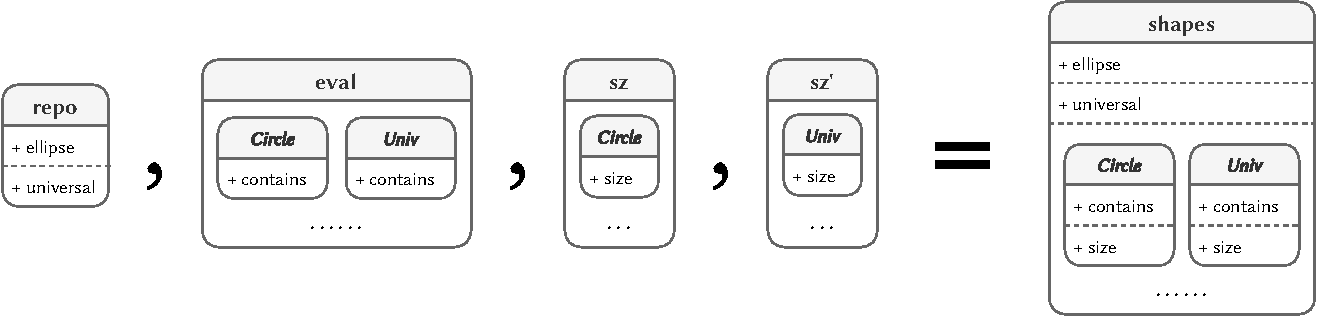
\includegraphics[width=\textwidth]{merge.pdf}
  \caption{A visualization of nested trait composition.} \label{fig:compose}
\end{figure}

\noindent
We provide the final semantic domain (\lstinline{Eval&Size}), as the type
argument, for the trait \lstinline{repo} and merge it with three other modularly
defined traits. The trait composition is called
\emph{nested}~\citep{bi2018essence} because not only different sets of
constructors, but also different semantics nested in the same constructor are
merged. In our case, both interpretations are available under the two sets of
language constructs after nested composition, as visualized in
\autoref{fig:compose}. Here, the language constructs and their semantics form a
two-level hierarchy of traits. Such composition of whole hierarchies can be
traced back to \emph{family polymorphism}~\citep{ernst2001family}. With this
powerful mechanism of nested composition, we can easily develop highly modular
\emph{product lines}~\citep{apel2013feature} of DSLs, where DSL features can be
composed \emph{à la carte}.

\subsection{Dependency Injection and Domain-Specific Optimizations} \label{sec:deps}

Now we illustrate CP's support for \emph{modular dependent interpretations}. We
skip the simpler example with \lstinline{text} and focus on the more interesting
example with \lstinline{isUniv} and \lstinline{isEmpty}. Similarly to the deep
embedding in Haskell in \autoref{sec:transform}, we define two compositional
traits \lstinline{chkUniv} and \lstinline{chkEmpty}:

\begin{lstlisting}
type IsUniv  = { isUniv:  Bool };
type IsEmpty = { isEmpty: Bool };

chkUniv = trait implements RegionSig<IsEmpty => IsUniv> => {
  (Univ         ).isUniv = true;
  (Outside     a).isUniv = a.isEmpty;
  (Union     a b).isUniv = a.isUniv || b.isUniv;
  (Intersect a b).isUniv = a.isUniv && b.isUniv;
  (Translate _ a).isUniv = a.isUniv;
  (Scale     _ a).isUniv = a.isUniv;
                _.isUniv = false;
};

chkEmpty = trait implements RegionSig<IsUniv => IsEmpty> => {
  (Empty        ).isEmpty = true;
  (Outside     a).isEmpty = a.isUniv;
  (Union     a b).isEmpty = a.isEmpty && b.isEmpty;
  (Intersect a b).isEmpty = a.isEmpty || b.isEmpty;
  (Translate _ a).isEmpty = a.isEmpty;
  (Scale     _ a).isEmpty = a.isEmpty;
                _.isEmpty = false;
};
\end{lstlisting}

\noindent
The first thing to note is that the sort of \lstinline{RegionSig} is
instantiated with two types separated by a fat arrow (\lstinline{=>}). This is
how we \emph{refine} interface types for dependency injection. For example,
\lstinline{chkUniv} does not implement \lstinline{RegionSig<IsEmpty>}, but we
assume the latter is available. The static type checker of CP guarantees that
\lstinline{chkUniv} is later merged with another trait that implements
\lstinline{RegionSig<IsEmpty>}. That is why we can safely use
\lstinline{a.isEmpty} when implementing \lstinline{(Outside a).isUniv}. The
second trait \lstinline{chkEmpty} is just the dual of \lstinline{chkUniv}. It is
hard to define such interpretations modularly in traditional approaches because
they are dependent, but we make them compositional via dependency injection.
Lastly, \lstinline{_.isUniv} and \lstinline{_.isEmpty} are \emph{default
patterns}, which compensate for the remaining constructors declared in the
interface. For example, \lstinline{_.isUniv = false} implies
\lstinline{Empty.isUniv = false} and \lstinline{Circle.isUniv = false}. Note
that in CP, for modularity, patterns are \emph{unordered}, unlike functional
languages like Haskell or ML. Therefore, default patterns are local to the
traits where they are used. These patterns can be understood as a concise way to
fill the missing cases in the local trait. 

Another thing worth noting is that dependency injection in compositional
embeddings is more modular than direct dependencies in deep embeddings because
the former does not refer to concrete implementations. For example, in the
compositional embedding above, \lstinline{chkUniv} only requires that the
dependent trait should implement the interface \lstinline{RegionSig<IsEmpty>}.
However, in the deep embedding (see \autoref{sec:mutual}), \lstinline{isUniv}
depends on the specific \lstinline{isEmpty} implementation.

\paragraph{Delegated method patterns.}
In some complicated transformations, nested pattern matching is required to
inspect smaller constructs. Nested pattern matching is not directly supported in
CP yet. However, there is a simple transformation that we can do whenever we
would like to have nested patterns:  we can delegate the inner tasks to other
methods whereby only top-level patterns are needed. We call such a technique
\emph{delegated method patterns}.

Concerning the nested pattern matching in \autoref{sec:nested}, we can implement
it with two mutually dependent methods. Since delegated method patterns are not
reused, the two methods are defined together for the sake of simplicity (but can
always be separated into two traits):

\begin{lstlisting}
type Eliminate Region = { eliminate: Region; delOutside: Region };

elim Region = trait [fself: RegionSig<Region>]
              implements RegionSig<Region => Eliminate Region> => {
  (Outside     a).eliminate = a.delOutside;
  (Union     a b).eliminate = Union a.eliminate b.eliminate;
  (Intersect a b).eliminate = Intersect a.eliminate b.eliminate;
  (Translate v a).eliminate = Translate v a.eliminate;
  (Scale     v a).eliminate = Scale v a.eliminate;
           [self].eliminate = self;

  -- delegated method patterns:
  (Outside a).delOutside = a.eliminate;
       [self].delOutside = Outside self.eliminate;
};
\end{lstlisting}

\noindent The translation from nested pattern matching to delegated method
patterns is straightforward. Our code lifts nested patterns
(\lstinline{Outside (Outside a)}) to top-level delegated patterns. In this way,
we do not change the underlying algorithm at all. This is in contrast with
approaches like tagless-final embeddings that, as discussed in
\autoref{sec:transform}, seem unable to directly support nested patterns,
requiring different algorithms to achieve the same goal. Though our approach is
not as convenient as deep embeddings, it is noteworthy that we can just write
the original algorithm \emph{modularly}.

If we add new language constructs in the future, it is easy to augment the
traits with more top-level patterns, but extending nested patterns is difficult
because there is no name to denote the \emph{extension point}. With delegated
method patterns, the method name \lstinline{delOutside} offers an extension
point for additional cases in the nested pattern matching. For instance, if we
wish for an extension supporting a new kind of region and a special case for
eliminating a region outside this kind of region
(\lstinline{eliminate (Outside (SomeRegion params))}), we can have a trait with
a method pattern of the following form, modularly defined in another trait:

\begin{lstlisting}
(SomeRegion params).delOutside = ...
\end{lstlisting}

\noindent
Although we believe that the design of CP can be improved to better support
similar logic to nested patterns, there are important differences between
traditional (closed) forms of pattern matching and open pattern
matching~\citep{zhang2020castor}. For instance, patterns in CP are unordered for
compositionality, but the order of patterns matters in conventional pattern
matching. Thus the design of improved language support for nested patterns in
CP, which could make the use of delegated method patterns more convenient,
requires further research and is left for future work.

\paragraph{Linguistic reuse after transformations.}
Before finishing the discussion of modular transformations, let us revisit CP's
support for linguistic reuse: can we still have meta-language optimizations for
free after complicated transformations? The answer is yes. To demonstrate this
point, we can modify the definition of \lstinline{circles} in
\autoref{sec:sharing} to have an inefficient
\lstinline{Outside (Outside (Circle 1.0))}. As usual, we compose all the
necessary traits together to make sure no dependencies are missing:

\begin{lstlisting}
test' = new sharing' @(Size & Eliminate Size) , sz , sz' , elim @Size;
test'.circles.eliminate.size
\end{lstlisting}

\noindent
The evaluation terminates as quickly as before, meaning that meta-language
optimizations are still performed even after a transformation.

We should remark that there are limits to the form of implicit sharing (and
linguistic reuse) that shallow embeddings or compositional embeddings provide.
For both shallow and compositional embeddings, implicit sharing will not work if
the interpretation is a function, such as \lstinline{contains}. In such cases,
the sharing is still lost. Nevertheless, implicit sharing is an important
feature that is often exploited in shallow DSLs. With compositional embeddings,
we can take this idea further and make it work even after some transformations
and optimizations have been applied. Moreover, it is also possible to adopt
solutions with explicit sharing by modeling a \lstinline{Let} construct in the
DSL.

\subsection{A Detailed Comparison between Different Embedding Approaches} \label{sec:comparison}

\begin{table}[b!]
\caption{A detailed comparison between different embedding approaches.} \label{tab:comparison}
\centering
\begin{tabular}{*{6}{c}}
\toprule
                                       &\textsc{Shallow}& \textsc{Deep} &\textsc{Hybrid}& \textsc{Poly.}& \textsc{Comp.}\\
\midrule \midrule
Transcoding free                       &    \CIRCLE     &    \CIRCLE    &    \Circle    &    \CIRCLE    &    \CIRCLE    \\
Linguistic reuse                       &    \CIRCLE     &    \Circle    &    \CIRCLE    &    \CIRCLE    &    \CIRCLE    \\
Language construct extensibility       &    \CIRCLE     &    \Circle    &\LEFTcircle$^1$&    \CIRCLE    &    \CIRCLE    \\
Interpretation extensibility           &    \Circle     &    \CIRCLE    &    \CIRCLE    &    \CIRCLE    &    \CIRCLE    \\
Transformations and optimizations      &    \Circle     &    \CIRCLE    &    \CIRCLE    &\LEFTcircle$^2$&\LEFTcircle$^2$\\
Linguistic reuse after transformations &    \em n/a     &    \Circle    &    \Circle    &    \CIRCLE    &    \CIRCLE    \\
Modular dependencies                   &    \Circle     &\LEFTcircle$^3$&\LEFTcircle$^3$&    \Circle    &    \CIRCLE    \\
Nested pattern matching                &    \Circle     &    \CIRCLE    &    \CIRCLE    &    \Circle    &\LEFTcircle$^4$\\
\bottomrule
\end{tabular}
\vskip 1ex
{\footnotesize
  $^1$ The extensibility of language constructs is limited or precludes exhaustive pattern matching.\\
  $^2$ Transformations require some ingenuity and are sometimes awkward to write.\\
  $^3$ Dependencies do not require code duplication but still refer to concrete implementations.\\
  $^4$ Nested pattern matching is implemented as delegated method patterns.\\
}
\end{table}

\noindent
In \autoref{tab:comparison}, we compare existing embedding approaches in the
literature with compositional embeddings. Shallow and deep embeddings have been
discussed in detail in \autoref{sec:embed}, and the table summarizes the points
that we have made. Hybrid
approaches~\citep{rompf2012scala,svenningsson2015combining,jovanovic2014yinyang}
employ both embeddings together. However, transcoding from shallow to deep is
generally needed, as both shallow and deep implementations must coexist side by
side. There is a clear boundary between the two parts: linguistic reuse is
available only in the shallow part, while complex transformations are available
only in the deep part. Therefore, it is still hard to exploit host-language
features after transformations. In work by
\citeauthor{svenningsson2015combining}, we cannot add more constructs to the
deeply embedded AST but can only extend shallowly embedded syntactic sugar. In
Scala, if \emph{open} case classes~\citep{emir2007matching} are used for deep
embeddings, ASTs are also extensible but do not ensure the exhaustiveness of
pattern matching. Compositional embeddings offer a unified approach directly
capable of all these functionalities.

\paragraph{Non-modular dependencies in modular embeddings.}
Polymorphic embeddings~\citep{hofer2008polymorphic}, tagless-final
embeddings~\citep{carette2009finally,kiselyov2010typed}, and object
algebras~\citep{oliveira2012extensibility} (denoted as \textsc{Poly.} in the
table) also provide a unified encoding where most advantages of shallow and deep
embeddings are available. However, they cannot deal with dependencies modularly.
Let us take tagless-final embeddings for example, which can also be implemented
in Haskell. We refer curious readers to \autoref{sec:tagless} for the complete
code.

In the tagless-final embedding, region constructors are defined in a type class
instead of a closed algebraic data type, and \lstinline{Size} can be modularly
defined as an instance of the type class since it has no dependency:

\noindent
\begin{minipage}{0.48\textwidth}
\begin{lstlisting}[language=Haskell,deletekeywords={union,intersect}]

class RegionHudak repr where
  circle    :: Double -> repr
  outside   :: repr -> repr
  union     :: repr -> repr -> repr
  intersect :: repr -> repr -> repr
  translate :: Vector -> repr -> repr
\end{lstlisting}
\end{minipage}%
\begin{minipage}{0.52\textwidth}
\begin{lstlisting}[language=Haskell,deletekeywords={union,intersect}]
newtype Size = S { size :: Int }
instance RegionHudak Size where
  circle      _ = S 1
  outside     a = S $ a.size + 1
  union     a b = S $ a.size + b.size + 1
  intersect a b = S $ a.size + b.size + 1
  translate _ a = S $ a.size + 1
\end{lstlisting}
\end{minipage}

\noindent
But how about the textual representation? As a first try, we might write:

\begin{lstlisting}[language=Haskell]
newtype Text = T { text :: String }
instance RegionHudak Text where
  circle  r = T { text = "circular region of radius " ++ show r }
  outside a = T { text = "outside a region of size " ++ show a.size }
  ......
\end{lstlisting}

\noindent
Unfortunately, we will get a type error concerning \lstinline{a.size} because
\lstinline{a} has type \lstinline{Text} and thus does not contain a field named
\lstinline{size}. Once we need operations that have some dependencies on other
operations, we get into trouble!

A simple workaround is to pack the two operations together and duplicate the
code of size calculation. We have already described this approach for shallow
embeddings in \autoref{sec:transform}, and the same workaround works for
tagless-final embeddings:

\begin{lstlisting}[language=Haskell,deletekeywords={union,intersect}]
data SizeAndText = ST { size :: Int, text :: String }
instance RegionHudak SizeAndText where
  circle  r = ST { size = 1, text = "circular region of radius " ++ show r }
  outside a = ST { size = a.size + 1
                 , text = "outside a region of size " ++ show a.size }
  ......
\end{lstlisting}

\noindent However, this is not modular since we have to duplicate code for size
calculation, even though the size calculation is completely independent of the
textual representation. If we have another operation that depends on
\lstinline{size}, we have to repeat the same code even again. This workaround is
an \emph{anti-pattern}, which violates basic principles of software engineering.
Duplicating code every time we need a dependent interpretation is a serious
problem since dependencies are extremely common. Nearly all non-trivial code
will have dependencies. In functional programming, it is common to have
functions defined by pattern matching that call other functions defined by
pattern matching, which is where an important form of dependencies appears. As
shown in \autoref{sec:fancier}, some workarounds that avoid code duplication in
Haskell are possible, but this typically comes at the cost of more code and the
use of advanced language features. 

\paragraph{The third dimension of the expression problem.}
In essence, dependencies are a third dimension that is not discussed in the
formulation of the expression problem by \citet{wadler1998expression}: whether
dependencies require code duplication or not. If we take this into
consideration, we can get a revised formulation of the expression problem, where
instead of only two dimensions, we have a third dimension that evaluates the
ability of an approach to deal with dependencies. With this extra dimension
taken into account, what we get is \autoref{tab:3d}. While tagless-final or
other embeddings address the two original dimensions of extensibility modularly,
they become non-modular with respect to dependencies, and programming with
dependencies becomes significantly more awkward compared to conventional FP or
OOP.

\begin{table}[b]
\caption{A briefer comparison regarding the three dimensions of the expression problem.} \label{tab:3d}
\centering
\begin{tabular}{*{5}{c}}
\toprule
                    &     FP  &     OOP &\textsc{Poly.}&\textsc{Comp.}\\
\midrule \midrule
New constructs      & \Circle & \CIRCLE &      \CIRCLE &      \CIRCLE \\
New functions       & \CIRCLE & \Circle &      \CIRCLE &      \CIRCLE \\
\emph{Dependencies} & \CIRCLE & \CIRCLE &      \Circle &      \CIRCLE \\
\bottomrule
\end{tabular}
\vskip 1ex
{\footnotesize \CIRCLE \; no code duplication \qquad
               \Circle \; code duplication needed}
\end{table}

Note that we are not the first to observe the problem with dependencies. The
problem above is known and discussed widely in the literature. In the context of
polymorphic embeddings, \citet{hofer2008polymorphic} face the problem of
dependencies and use the non-modular approach with tuples. Later
\citet{hofer2010modular} adopt an extensible visitor pattern to improve
modularity, but this results in much more boilerplate code. In his lecture notes
on tagless-final interpreters, \citet{kiselyov2010typed} has a strong focus on
discussing how to write non-compositional interpretations, which basically
include operations with dependencies and nested pattern matching. He shows that
non-compositional programs can often be rewritten as programs that use contexts
instead. The problem of modular dependencies has been widely discussed within
the context of object algebras. Most recently,
\citet{zhang2017evf,zhang2020castor} propose solutions to the problem using
meta-programming techniques. \citet{zhang2019shallow} further explore modular
solutions in both Scala and Haskell, but their approaches still require a lot of
boilerplate code. In Scala, it is due to a lack of language support for nested
composition, whereas Haskell needs to encode dependencies via type classes to
modularize dependent interpretations (see \autoref{sec:fancier} for a similar
solution). The drawbacks of the existing solutions above motivate the design of
CP and compositional embeddings.

\paragraph{Transformations.}
It is widely believed that transformations and optimizations are much easier to
write in deep embeddings~\citep{jovanovic2014yinyang,scherr2014implicit}. We
agree that it requires some ingenuity and is sometimes awkward to write complex
transformations in compositional embeddings, but \citet{kiselyov2010typed} has
demonstrated that several challenging transformations can be written with
tagless-final embeddings. Compositional programming is a generalization of such
forms of embeddings, and therefore all the transformations are possible with
tagless-final embeddings are also possible in CP. Even for structurally
non-local transformations, we can instantiate a sort with a function type (e.g.
\lstinline{RegionSig<Ctx->Region>}) and pass down the context when traversing
the AST. Such contextual transformations can also be modular with the help of
\emph{polymorphic contexts}~\citep{zhang2021compositional}. We have implemented
an example of common subexpression elimination inspired by
\citet{kiselyov2011implementing} (which can be found in our online
implementation). Both our code and \citeauthor{kiselyov2011implementing}'s are
not fully modular with respect to an auxiliary data structure (his
implementation relies on a closed algebraic data type). In our case, this is
because nested composition for recursive types is currently not supported, which
relies on future theoretical progress of reconciling distributive subtyping and
recursive types. Nevertheless, our approach is less entangled than tagless final
embeddings since we can handle dependent transformations modularly.

\section{\ExT: A DSL for Document Authoring} \label{sec:dsl}

We have presented the advantages of compositional embeddings using a relatively
small DSL. One may wonder if our approach scales to larger DSLs. As our answer
to this question, we developed a larger DSL for document authoring called \ExT.

\ExT applies compositional embeddings to a document DSL, inspired by \LaTeX{}
and Scribble~\citep{flatt2009scribble}. We have also done minor syntactic
extensions to the CP language to support writing documents more naturally. Since
documents usually involve large portions of text, it would be awkward to write
such portions of text using string literals adopted by most programming
languages. CP does not yet have facilities for syntactic extension that other
languages (e.g. Racket, Haskell, or Coq) offer, so we have extended the parser
directly. Thus, CP parses some document-specific syntax and desugars it to
compositionally embedded fragments during parsing. Such a generative approach is
similar to Racket macros~\citep{ballantyne2020macros} and Template
Haskell~\citep{sheard2002template}, which provide more flexible facilities for
performing such desugaring. Nevertheless, the surface syntax of \ExT is
essentially a set of lightweight syntactic sugar for its underlying
compositional embeddings (similar, for instance, to Scribble in Racket).

\subsection{Design Goals and Non-Goals} \label{sec:goals}

There are already a large number of document DSLs, so why shall we create yet
another one? We explain why by identifying important design goals and non-goals
of \ExT.

\paragraph{A document language for the web.}
A first goal is to have a lightweight but powerful document language tailored
mostly for the web. We view \ExT as an alternative to Wikitext~\citep{wikitext},
the markup language used by Wikipedia, which shares similar goals. Similar to
Wikipedia pages, users can directly edit \ExT documents on a web page. But
different from Parsoid~\citep{parsoid}, the official Wikitext parser that runs
on the server side, our implementation can directly render documents on the
browser side.

\paragraph{General-purpose computation.}
The majority of existing document DSLs (e.g. CommonMark~\citep{mark},
Textile~\citep{textile}, and reStructuredText~\citep{rst}) have a fixed set of
language features and do not provide general-purpose computation. For instance,
we may want to compute a table from some data, like a table listing the largest
cities in descending order of population. For such kinds of tasks, it is useful
to have mechanisms for general-purpose computation that allow us to
\emph{compute} documents rather than manually write them.

Although some other document DSLs provide language constructs that enable some
computation, they still have significant limitations. For instance, Wikitext
provides templates, which play a role similar to functions in conventional
programming languages. However, templates cannot perform arbitrary computation
as CP does. The documentation says,\footnote{The sentence is extracted from
\url{https://en.wikipedia.org/wiki/Wikipedia:TEMPLATE_LOOP}.} ``A template can
call itself but will stop after one iteration to prevent an infinite loop.'' In
other words, templates by themselves are incapable of recursion or loops, but in
practice, loops are often needed in Wikipedia. For instance,
\lstinline|{{loop}}| has been used on approximately 99,000 pages.\footnote{The
number of transclusions (99,000 as of July 2022) is shown at
\url{https://en.wikipedia.org/wiki/Template:Loop}.} A Lua extension was
introduced to bypass such restrictions, and the widely-used template
\lstinline|{{loop}}| invokes \lstinline{string.rep} in Lua. Instead of handing
it over to an external language, CP directly supports functions, and thus
general-purpose computation is easily done in \ExT, including recursion. 

\paragraph{Static type checking.}
In contrast to many document languages, CP and \ExT are statically type checked.
Static type checking enables us to detect some errors that may arise when
processing documents. In applications like wikis, it is very frequent that we
need some form of structured data. States or cities, for example, may have
infoboxes associated with them that list several pieces of data, such as areas,
populations, official languages, etc. Using simple text to store such data can
easily lead to simple errors. In addition, if we want to enable computed
information as previously described, then it is useful to have a type system
that allows us to write functions that take a well-defined form of structured
data. Most document languages that we know of, including Wikitext, \LaTeX{}, and
Scribble, are not statically typed. We will discuss some examples where static
typing is helpful in \ExT in \autoref{sec:typing}.

\paragraph{Extensible meta-programming and customizability.}
A benefit of modeling a DSL as an algebraic data type or a compositional
interface is that we can easily write meta-functions over the abstract syntax of
the DSL. For instance, in the context of documents, such meta-functions could
include rendering to various backends (such as \LaTeX{} or HTML) or computing a
table of contents based on the document tree. In many external DSLs, such
meta-functions are typically much harder to write, requiring us to directly
modify the implementation. However, by embedding a DSL, the host language can
act as a meta-language for the DSL and allow us to easily write meta-programs,
for instance, as functions to process the AST by pattern matching.

In addition, the extensibility of compositional embeddings enables a form of
extensible meta-programming: not only can we write meta-functions, but those
meta-functions can be extended later to cater for new language constructs
modularly defined by users. This enables DSL users to \emph{modularly} extend
the basic document language to add their own extensions, including infoboxes,
vector graphics, etc. While Scribble does provide good facilities for syntactic
extension and meta-programs, the document structure is fixed~\citep{scribble},
so the DSL is not fully extensible. In short, \ExT is designed to be extensible
and highly customizable by users. 

\paragraph{Non-goals.}
Currently, our implementation of CP is a fairly naive call-by-need interpreter,
so the performance of \ExT is not competitive with well-established tools like
\LaTeX. Furthermore, unlike \LaTeX, which has extensive libraries developed over
many years, there are no third-party libraries for \ExT. Thus, \ExT is
\emph{not} yet production-ready. Another non-goal is security. Since we never
sanitize user-generated HTML, it is easy to perform JavaScript code injection on
our website. It is off-topic to consider how to ensure web security here.

\subsection{Syntax Overview}

\begin{figure}
\begin{subfigure}{0.58\textwidth}
\begin{Verbatim}[fontsize=\small]
\Section[
  Welcome to
  \Href("https://plground.org")[PLGround]!
]
\Bold[CP] is a \Emph[compositional]
programming language. \\\\
There are \(1+1+1+1) key concepts in CP:
\Itemize[
  \Item[Compositional interfaces;]
  \Item[Compositional traits;]
  \Item[Method patterns;]
  \Item[Nested trait composition.]
]
\end{Verbatim}
\caption{\ExT code.}
\end{subfigure}%
\begin{subfigure}{0.42\textwidth}
\scalebox{0.8}{\begin{minipage}{\textwidth}
\section*{%
  Welcome to
  \href{https://plground.org}{PLGround}!
}
\textbf{CP} is a \emph{compositional}
programming language. \\\\
There are 4 key concepts in CP:
\begin{itemize}
\item Compositional interfaces;
\item Compositional traits;
\item Method patterns;
\item Nested trait composition.
\end{itemize}
\end{minipage}}
\vspace{1em}
\caption{Rendered document.}
\end{subfigure}
\caption{A sample document illustrating \ExT syntax.} \label{fig:example}
\end{figure}

\noindent
The syntax of \ExT is designed for easy document authoring, as shown in
\autoref{fig:example}. It is reminiscent of \LaTeX, but still has significant
differences. The similarity is that plain text can be directly written while
commands start with a backslash. But we choose different brackets for command
arguments:

\begin{itemize}
\item \Verb|\Cmd[...]| encloses document arguments. Square brackets indicate
      that a sequence of nested elements is recursively parsed. (Most commands
      in \autoref{fig:example} are in such a form, for example,
      \lstinline|\Section| and \lstinline|\Bold|.)
\item \Verb|\Cmd(...)| encloses positional arguments. Parentheses indicate that
      the whole construct is desugared to function application.
      (\lstinline|\Href| in \autoref{fig:example} is an example.)
\item \Verb|\Cmd{...}| encloses labeled arguments. Braces indicate that these
      arguments are wrapped in a record. (As mentioned in \autoref{sec:typing},
      \lstinline|\Line{ x1 = 0.0; y1 = 0.0; x2 = 4.6; y2 = 4.8 }| uses this form
      to distinguish different attributes.)
\end{itemize}

\noindent
A command can be followed by an arbitrary number of different arguments in any
order. This syntax is more flexible than the fixed form
\lstinline|@op[...]{...}| in Scribble. Although both arguments are optional in
Scribble, they can neither occur more than once nor be shuffled. In addition,
there are two more useful \ExT constructs. One is string interpolation with the
form \lstinline{\(...)}, which has exactly the same syntax as the Swift
programming language. We can see an example of string interpolation in
\autoref{fig:example}: \lstinline|\(1+1+1+1)|. It will be desugared to
\lstinline{Str (toString (1+1+1+1))}. This example will execute the code, which
computes ``4'', and its string form will be interpolated in the document. The
other construct is double backslashes (\lstinline{\\}), a shorthand for newline,
which is borrowed from \LaTeX. In \ExT, it is equivalent to the
\lstinline{\Endl} command. There is also an example in \autoref{fig:example},
which inserts a newline character between the first and second sentences in the
body. 

\paragraph{Desugaring.}
As mentioned earlier, all \ExT constructs are desugared to normal CP code. For
example, the following two expressions are equivalent (the document DSL is
enclosed within backticks):

\begin{lstlisting}
`\Entry("id"){ hidden = true; level = 1 }[This entry is \Emph[hidden]]`
-- is desugared to:
Entry "id" { hidden = true; level = 1 } (Comp (Str "This entry is ")
                                              (Emph (Str "hidden")))
\end{lstlisting}

\noindent Here, \lstinline{Comp} and \lstinline{Str} are two special commands
that are assumed to be implemented by library authors. \lstinline{Comp} is used
for composing an AST of document elements, while \lstinline{Str} is for plain
text.

\paragraph{Specification.}
The grammar of \ExT can be summarized in whole as follows (\lstinline{<arg>*}
means that \lstinline{<arg>} may occur zero or more times):

\begin{Verbatim}[fontsize=\small]
<doc> ::= <str> | "\" <esc>
<esc> ::= <cmd> <arg>* | "(" <exp> ")" | "\"
<arg> ::= "[" <doc> "]" | "(" <exp> ")" | "{" <rcd> "}"

<str> ::= text without "\" and "]"
<cmd> ::= identifier
<exp> ::= expression
<rcd> ::= record fields
\end{Verbatim}

\subsection{Extensible Commands with Multi-Backend Semantics}

\ExT is so flexible that only a few commands are really compulsory. Additional
commands and their semantics can be extended as needed. At the very beginning,
we only need to define the aforementioned three special commands:

\begin{lstlisting}
type DocSig<Element> = {
  Comp: Element -> Element -> Element;
  Str:  String -> Element;
  Endl: Element;
};
\end{lstlisting}

\noindent
However, for rich text in real-world documentation, these commands are not
sufficient for various document elements. Adding new commands and their
semantics is not hard at all in compositional embeddings, like what we have done
in \autoref{sec:syntax} and \autoref{sec:semantics}. Language interfaces can be
separately declared and then intersected with each other. Besides extensible
commands, their semantics are also retargetable. We can modularly create
different traits for different backends, such as HTML and \LaTeX:

\begin{lstlisting}
type HTML = { html: String };
html = trait implements DocSig<HTML> => {
  (Comp l r).html = l.html ++ r.html;
  (Str    s).html = s;
  (Endl    ).html = "<br>";
};

type LaTeX = { latex: String };
latex = trait implements DocSig<LaTeX> => {
  (Comp l r).latex = l.latex ++ r.latex;
  (Str    s).latex = s;
  (Endl    ).latex = "\\\\";
};
\end{lstlisting}

\begin{figure}
  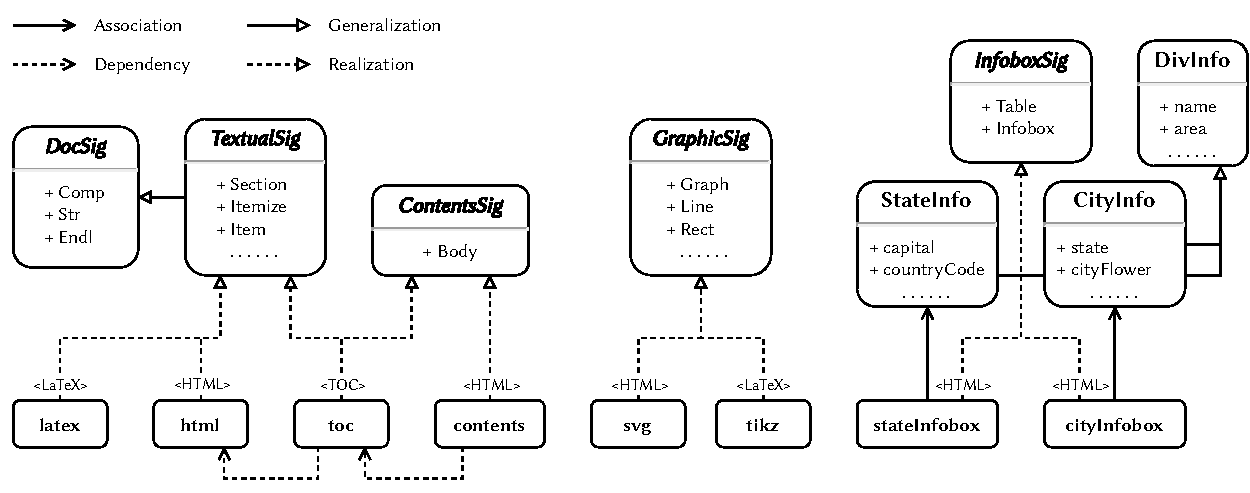
\includegraphics[width=\textwidth]{libraries.pdf}
  \caption{A simplified diagram of \ExT components.} \label{fig:diagram}
\end{figure}

\paragraph{The components of \ExT.}
We have implemented several extensions of \ExT, as shown in
\autoref{fig:diagram}. In the upper part of the diagram, the capitalized names
in a bold italic font (e.g. {\small \sffamily \bfseries \itshape DocSig}) are
compositional interfaces, while those in a bold upright font (e.g. {\small
\sffamily \bfseries DivInfo}) are normal types. The smaller boxes at the bottom
of the diagram are compositional traits. They implement different interfaces
with the sorts specified on the dashed arrows, (e.g. {\small \sffamily <HTML>}).
Specifically, \lstinline{TextualSig} adds a set of common commands for rich
text, such as \lstinline{Section}, \lstinline{Itemize}, \lstinline{Item}, etc.
It extends \lstinline{DocSig} and targets both HTML and \LaTeX.
\lstinline{GraphicSig} is used to draw vector graphics (including lines,
rectangles, circles, etc.), which are supported in HTML and \LaTeX{} via SVG and
Ti\emph{k}Z respectively. \lstinline{InfoboxSig} targets only HTML and adds
Wikipedia-like infoboxes (containing, for instance, information about areas and
populations of states or cities). All these compositional interfaces and traits
can be combined to form a heterogeneous composition. Notably, the implementation
of \lstinline{ContentsSig}, which is used to generate a table of contents,
introduces some non-trivial dependencies (see \autoref{sec:minipedia}).

\subsection{Static Typing} \label{sec:typing}

A major difference of \ExT from other document DSLs is that it is statically
type checked. With static typing, potential type errors can be detected ahead of
time, saving users' time for debugging. For example, when drawing a line using
SVG, we need to use the \lstinline{<line>} element with four numeric coordinates
(\lstinline{x1}, \lstinline{y1}, \lstinline{x2}, and \lstinline{y2}). However,
since additional information of an SVG element is represented as XML attributes,
all of the coordinates have to be quoted as strings instead of numbers. Only
after rendering it with a web browser and opening developer tools can one check
if attributes are valid. In \ExT, we model the line construct like this:

\begin{lstlisting}
type GraphicSig<Graphic> = {
  Line: { x1: Int; y1: Int; x2: Int; y2: Int } -> Graphic;
  -- and more constructors
};
\end{lstlisting}

\noindent
Before rendering lines via SVG, the types of arguments are checked against the
language interface, and invalid values are rejected in advance. Note that the
error messages are reported in terms of the \ExT surface syntax, which is more
friendly to users than some meta-programming techniques, where errors are
reported in terms of the generated code.

When modeling infoboxes and bibliography in \autoref{sec:minipedia}, we also
make use of data types to represent structured information. For example, we use
\lstinline{DivInfo} to model common information required by all political
divisions, as well as two specific types for states and cities respectively,
which extend \lstinline{DivInfo} using intersection types:

\noindent
\begin{minipage}{0.28\textwidth}
\begin{lstlisting}
type DivInfo = {
  name:       String;
  area:       Int;
  population: Int;
  languages: [String];
};
\end{lstlisting}
\end{minipage}
\hfill
\begin{minipage}{0.29\textwidth}
\begin{lstlisting}
type StateInfo =
       DivInfo & {
  countryCode: String;
  religions:  [String];
  -- and more fields
};
\end{lstlisting}
\end{minipage}
\hfill
\begin{minipage}{0.27\textwidth}
\begin{lstlisting}
type CityInfo =
      DivInfo & {
  cityFlower: String;
  timeZone:   String;
  -- and more fields
};
\end{lstlisting}
\end{minipage}

\noindent In this case, there is quite a bit of structure in the data. It
statically describes what fields are allowed and what types these fields have. 

\section{Evaluation of Compositionally Embedded \ExT}

In this section, we describe three applications of CP, compare them with
alternatives in other document languages, and evaluate the use of
compositionally embedded \ExT for the three applications.

\subsection{Minipedia} \label{sec:minipedia}

Minipedia is a mini document repository of states and cities, which reconstructs
a small portion of Wikipedia. Minipedia currently contains pages of the world's
ten smallest countries and their capitals, as well as a structured data file
storing all facts about them used for infoboxes. There are also pages consisting
of sorted tables of microstates by area or population, which are computed using
the information stored in the data file. Minipedia comprises over 4,000 lines of
code in total, most of which is accounted for by document pages. Among the rest,
the data file and \ExT libraries account for around 300 and 200 lines of code,
respectively.

\paragraph{Drawbacks of Wikipedia.}
Compared to our approach, Wikipedia and its markup language Wikitext have
several drawbacks, as partly mentioned in \autoref{sec:goals}:
\begin{itemize}
\item All data in Wikitext is in string format. Wikitext does not differentiate
      data types like \lstinline{Int}, \lstinline{Bool}, etc. This makes type
      errors remain uncaught in Wikipedia infoboxes. For example, in the infobox
      of a country, the population field can be changed to a non-numeric
      meaningless value, and Wikipedia will not warn the editor at all.
\item Statistical data is manually written on every Wikipedia page. This can
      easily result in data inconsistency for the same field across different
      pages, and even for different places on the same page. For example, the
      population size on a country page is often different from that in a
      statistical page listing all countries by population, owing to different
      data sources.
\item Wikitext provides user-defined templates as a reusable unit of document
      fragments. They can be parametrized and play a similar role to functions.
      However, they do not natively support general-purpose computation like
      recursion. Along with the Lua extension and parser functions, Wikitext
      offers some computational power to Wikipedia documents, but it is not as
      easy to use as \ExT is.
\end{itemize}

\paragraph{Type safety and data consistency.}
Minipedia has a structured data file containing the information of states and
cities, each piece of which is modeled as a record. The record types have been
shown in \autoref{sec:typing}. Every record for states or cities is type checked
against their corresponding types and collected in two arrays in the data file:

\noindent
\begin{minipage}{0.5\textwidth}
\begin{lstlisting}
tuvalu = {
  name       = "Tuvalu";
  area       = 26;
  population = 10645;
  -- and more fields
} : StateInfo;
states = [tuvalu; {- and more -}];
\end{lstlisting}
\end{minipage}%
\begin{minipage}{0.5\textwidth}
\begin{lstlisting}
funafuti = {
  name       = "Funafuti";
  area       = 2;
  population = 6320;
  -- and more fields
} : CityInfo;
cities = [funafuti; {- and more -}];
\end{lstlisting}
\end{minipage}
\smallskip

\noindent Such a centralized data file forces different documents to read from
the same data source and prevents data inconsistency. Not only infoboxes but
also computed documents like sorted lists of countries can be created using the
information from the data file. Moreover, if the area of Tuvalu, for example, is
assigned a string value, there will be a type error before rendering.

\paragraph{Writing Minipedia pages in \ExT.}
Writing Minipedia documents is enabled by the \ExT libraries shown in
\autoref{fig:diagram}. Different features of \ExT are defined in different
libraries, and we can import whatever libraries we want when writing a document.
For Minipedia, we only need HTML-related libraries. There are two modes for
document authoring in Minipedia: ``doc-only'' and ``program''. In the
``doc-only'' mode, with required libraries specified, documents are written
directly in \ExT without any wrapping code in CP, as shown in
\autoref{fig:example}. In the ``program'' mode, a document is created
programmatically in a mixture of CP and \ExT code. This mode makes
general-purpose computation easier to write in a document.

For example, a sorted table of the smallest countries by area demonstrates
general-purpose computation in the ``program'' mode. The program begins with an
\lstinline{open} directive, which imports definitions from the specified
libraries. We sort the array of countries imported from \lstinline{Database}
using a predefined function \lstinline{sort} and then iterate it to generate
\ExT code. As explained in \autoref{sec:sharing}, we use self-type annotations
to inject dependencies on the library commands. The intersection type
\lstinline{DocSig<T>&TableSig<T>} allows \ExT commands from both compositional
interfaces to be used in the trait \lstinline{doc}:

\begin{lstlisting}
open LibDoc;
open LibTable;
open Database;

sortedStates = sort states;
doc T = trait [self: DocSig<T>&TableSig<T>] => {
  table = letrec rows (i: Int): T = if i == 0 then `\Trow[
      \Theader[No.]   \Theader[Country]      \Theader[Area (km^2)]
    ]` else let state = sortedStates!!(i-1) in `\rows(i-1) \Trow[
      \Tdata[\(i+1)]  \Tdata[\(state.name)]  \Tdata[\(state.area)]
    ]` in `\Tbody[ \rows(#sortedStates) ]`;
};
document = new doc @HTML , html , table;
document.table.html
\end{lstlisting}

\paragraph{Adding a table of contents (TOC).}
We have introduced how to write Minipedia pages using \ExT libraries, but now
let us go back and see how we implement a \ExT library. The library of TOC adds
a new command \lstinline{\Body[...]}, which prepends a TOC to the document body.
The difficulty here is that HTML rendering depends on the TOC, whereas the TOC
in turn depends on the HTML rendering of section (and sub$^n$section) titles. As
we have demonstrated in \autoref{sec:deps}, we can modularly tackle such complex
dependencies by refining the interface types:

\begin{lstlisting}
type ContentsSig<Element> = { Body: Element -> Element };
type TOC = { toc: String };

contents = trait implements ContentsSig<TOC => HTML> => {
  [self]@(Body e).html = self.toc ++ e.html;
};
toc = trait implements TextualSig<HTML => TOC> & ContentsSig<TOC> => {
  (Comp        l r).toc = l.toc ++ r.toc;
  (Section       e).toc = listItem 0 e.html;
  (SubSection    e).toc = listItem 1 e.html;
  (SubSubSection e).toc = listItem 2 e.html;
  (Body          e).toc = "<ul>" ++ e.toc ++ "</ul>";
                  _.toc = "";
};
\end{lstlisting}

\noindent With \lstinline{TOC} specified in \lstinline{ContentsSig<TOC => HTML>}
and the self-reference specified in \lstinline{[self]}, we can call
\lstinline{self.toc} to generate a TOC when rendering HTML. Similarly, we can
call \lstinline{e.html} when generating the TOC since the interface type is
refined. A minor remark is that \lstinline{listItem} is an auxiliary function to
generate an appropriate \lstinline{<li>} wrapping for a given nesting level.

\subsection{Fractals and Sharing}

In the second application, we briefly introduce how to implement computational
graphics like fractals in \ExT with the help of linguistic reuse. Fractal
drawing is all about repeating the same pattern. This drives us to exploit
meta-language sharing to avoid redundant computation. We have implemented
several well-known fractals, such as the Koch snowflake, the T-square, and the
Sierpiński carpet. For the sake of simplicity, we take the Sierpiński carpet as
an example:

\begin{lstlisting}
fractal T C = trait [self: DocSig<T> & GraphicSig<T><C> & ColorSig<C> & Draw T C] implements Draw T C => {
  draw {..} =
    let center = Rect { x = x + width/3; y = y + height/3;
                        width = width/3; height = height/3; color = White } in
    if level == 0 then center else
      let w = width/3 in let h = height/3 in let l = level-1 in
      let shared = draw { x = x; y = y; width = w; height = h; level = l } in
      `\Group(id)[
         \shared
           \Translate{x=w;y=0}(shared)
             \Translate{x=2*w;y=0}(shared)
         \Translate{x=0;y=h}(shared)
           \center
             \Translate{x=2*w;y=h}(shared)
         \Translate{x=0;y=2*h}(shared)
           \Translate{x=w;y=2*h}(shared)
             \Translate{x=2*w;y=2*h}(shared)
      ]`
};
\end{lstlisting}

\noindent We make variables shared via the \lstinline{let} expressions in CP.
There are many uses in the code above but, among them, \lstinline{shared}
accelerates fractal generation the most. The variable \lstinline{shared} is
later used eight times to constitute the repeating patterns in the Sierpiński
carpet. \lstinline{\Translate} is a command declared in \lstinline{GraphicSig}
for geometric translations. With automatic linguistic reuse in \ExT, we only
need to generate a pattern once instead of repeating it eight times. Besides the
efficiency in generating fractals, our implementation of \lstinline{\Translate}
makes use of the \lstinline{<use>} element in SVG to avoid the exponential
growth of output. Therefore, the duplication of SVG elements is also eliminated.
These optimizations are available for free thanks to the linguistic reuse in
compositional embeddings.

\subsection{Customizing Charts} \label{sec:charts}

In the last application, we illustrate how line charts and bar charts are
modularly rendered using external data. Charts can be rendered into a document
using the \ExT language and its support for vector graphics. What is interesting
about charts is that there are many alternative ways to present charts and
customize them. The flexibility of the CP language, in terms of modularity and
compositionality, is then very useful here. We will show how to adapt
traditional object-oriented design patterns for compositional embeddings when
modeling graphic components.

\paragraph{Charting stocks.}
Taking stock prices as an example, we have a separate file containing data from
big companies, as well as a few configuration items for chart rendering. The
configuration includes the choice between lines and bars, whether to show
borders or legends, what labels to display, and so on. Serving as an
infrastructure, a base chart is created with the drawing functions for the
caption and axes:

\begin{lstlisting}
type Base = { caption: HTML; xAxis: HTML; yAxis: HTML };
baseChart (data: [Data]) = trait implements Base => {
  caption = `...`;  xAxis = `...`;  yAxis = `...`;
};
\end{lstlisting}

\noindent
The simplified code above shows a rough sketch, where a base trait takes data as
its parameter and implements the base interface. However, it does not implement
the primary rendering function. As we have two options to visualize stock
prices, we leave the choice to the \textsc{Strategy}
pattern~\citep{gamma1995design}.

\paragraph{\textsc{Strategy} pattern.}
Since the configuration is unknown until run time, the rendering strategy cannot
be hard-coded in the base trait. Instead, we define two strategy traits
implementing the rendering, respectively for lines and bars. They constitute two
variants of the base chart. It is not the programmer but the configurator that
decides which variant of charts should be rendered. In the original
\textsc{Strategy} pattern, a chart object delegates to a desired strategy
object, to which its mutable field points. That mutable field can be changed
from clients who use the chart. In CP, we just need to merge the base trait with
the strategy we want, without the need for mutable references:

\begin{lstlisting}
type Render = { render: HTML };
lineStrategy = trait [self: Base] implements Render => {
  render = let lines = ... in `\xAxis \yAxis \lines \caption`
};
barStrategy = trait [self: Base] implements Render => {
  render = let bars = ... in `\xAxis \yAxis \bars \caption`
};
chart = baseChart data , if config.line then lineStrategy else barStrategy;
\end{lstlisting}

\noindent
After merging, \lstinline{chart} is still a \emph{reusable trait}. This is
impossible in traditional object-oriented languages, like Java, because they
lack a dynamic way to compose classes at run time. In contrast, such a dynamic
trait composition is ubiquitous in CP. It is also easy to add a new strategy,
like switching to pie charts, and merge the base trait with the new one instead.
If a client forgets to pick any strategy, the type checker will notify them
because the trait types before and after merging are different. Moreover,
another advantage of our approach over the original strategy pattern is that the
self-type annotations make methods in the base trait accessible to strategy
traits. So \lstinline{caption}, \lstinline{xAxis} and \lstinline{yAxis} are
directly shared with strategies, requiring no extra effort to pass them as
arguments when delegating. This remedies the ``communication overhead between
Strategy and Context'' caused by the original \textsc{Strategy}
pattern~\citep{gamma1995design}.

\paragraph{\textsc{Decorator} pattern.}
Besides the \textsc{Strategy} pattern, the \textsc{Decorator}
pattern~\citep{gamma1995design} is also adapted for CP. Since decorations are
also determined by external configuration at run time, we need a modular way to
add additional drawing processes to the chart trait dynamically. When multiple
decorators are enabled, their functionalities should be added. In the original
\textsc{Decorator} pattern, the decorator class should inherit the chart class
and be instantiated with a reference to a chart object. The decorator will store
the chart object as a field and forward all methods to it. In concrete
decorators, the rendering function will be overridden to add decorations. The
decorator pattern sounds complicated in traditional object-oriented programming,
but the same goal can be achieved easily in CP using the \emph{dynamic
inheritance} provided by CP:

\begin{lstlisting}
type Chart = Base & Render;
borderDecorator (chart: Trait<Chart>) = trait [self: Chart] implements Chart inherits chart => {
  override render = let sr = super.render in let border = ... in `\sr \border`
};
legendDecorator (chart: Trait<Chart>) = trait [self: Chart] implements Chart inherits chart => {
  override caption = let legends = ... in `\legends`
};
chart' = if config.border then borderDecorator chart else chart;
chart'' = if config.legend then legendDecorator chart' else chart';
\end{lstlisting}

\noindent
A decorator takes a chart trait as the argument and creates another trait
inheriting it dynamically. In the implementation, we can override any methods as
usual, and static type safety is still guaranteed. It is worth noting that, in
\lstinline{legendDecorator}, only \lstinline{caption} is overridden while
\lstinline{render} is just inherited. In the original \textsc{Decorator}
pattern, \lstinline{render} will never be conscious of the overridden
\lstinline{caption} since the decorator hands over control to \lstinline{chart}
after forwarding \lstinline{render}. This is partly why \citet{gamma1995design}
warn readers that ``a decorator and its component aren't identical''. However,
in CP, \lstinline{chart.render} can access the overridden \lstinline{caption}
through the late-bound self-reference. This solution makes our code clean and
easy to maintain.

\paragraph{True delegation via trait composition.}
The chart application shows how other aspects of the modularity of CP are
helpful to create highly customizable DSLs. We have shown how CP adapts and
simplifies object-oriented design patterns. In general, we avoid complicated
class hierarchies in the original versions and replace them with relatively
simple trait composition. It showcases that we can get rid of verbose design
patterns if a proper language feature fills in the gap. In both patterns,
component adaptation is needed at run time, so delegation is at the heart of the
challenges.

